%===============================================================================
% LaTeX sjabloon voor de bachelorproef toegepaste informatica aan HOGENT
% Meer info op https://github.com/HoGentTIN/latex-hogent-report
%===============================================================================

\documentclass[dutch,dit,thesis]{hogentreport}

% TODO:
% - If necessary, replace the option `dit`' with your own department!
%   Valid entries are dbo, dbt, dgz, dit, dlo, dog, dsa, soa
% - If you write your thesis in English (remark: only possible after getting
%   explicit approval!), remove the option "dutch," or replace with "english".


\usepackage{graphicx}
\graphicspath{ {./graphics/} }

%% Pictures to include in the text can be put in the graphics/ folder
\graphicspath{{graphics/}}

%% For source code highlighting, requires pygments to be installed
%% Compile with the -shell-escape flag!
\usepackage[section]{minted}
\usemintedstyle{solarized-light}
\definecolor{bg}{RGB}{253,246,227} %% Set the background color of the codeframe

%% Change this line to edit the line numbering style:
\renewcommand{\theFancyVerbLine}{\ttfamily\scriptsize\arabic{FancyVerbLine}}

%% Macro definition to load external java source files with \javacode{filename}:
\newmintedfile[javacode]{java}{
    bgcolor=bg,
    fontfamily=tt,
    linenos=true,
    numberblanklines=true,
    numbersep=5pt,
    gobble=0,
    framesep=2mm,
    funcnamehighlighting=true,
    tabsize=4,
    obeytabs=false,
    breaklines=true,
    mathescape=false
    samepage=false,
    showspaces=false,
    showtabs =false,
    texcl=false,
}

% Other packages not already included can be imported here

%%---------- Document metadata -------------------------------------------------
% TODO: Replace this with your own information
\author{Jules Vervaeke}
\supervisor{Koen Mertens}
\cosupervisor{Pascal Synaeve}
\title[]%
    {Integratie van Machine Learning aan taxonomie-systeem van PIMLayer, een vergelijkende studie tussen \newline verschillende aanbieders van Machine Learning as a Service}
\academicyear{\advance\year by -1 \the\year--\advance\year by 1 \the\year}
\examperiod{1}
\degreesought{\IfLanguageName{dutch}{Professionele bachelor in de toegepaste informatica}{Bachelor of applied computer science}}
\partialthesis{false} %% To display 'in partial fulfilment'
%\institution{Internshipcompany BVBA.}

%% Add global exceptions to the hyphenation here
\hyphenation{back-slash}

%% The bibliography (style and settings are  found in hogentthesis.cls)
\addbibresource{bachproef.bib}            %% Bibliography file
\addbibresource{../voorstel/voorstel.bib} %% Bibliography research proposal
\defbibheading{bibempty}{}

%% Prevent empty pages for right-handed chapter starts in twoside mode
\renewcommand{\cleardoublepage}{\clearpage}

\renewcommand{\arraystretch}{1.2}

%% Content starts here.
\begin{document}

%---------- Front matter -------------------------------------------------------

\frontmatter

\hypersetup{pageanchor=false} %% Disable page numbering references
%% Render a Dutch outer title page if the main language is English
\IfLanguageName{english}{%
    %% If necessary, information can be changed here
    \degreesought{Professionele Bachelor toegepaste informatica}%
    \begin{otherlanguage}{dutch}%
       \maketitle%
    \end{otherlanguage}%
}{}

%% Generates title page content
\maketitle
\hypersetup{pageanchor=true}

%%=============================================================================
%% Voorwoord
%%=============================================================================

\chapter*{\IfLanguageName{dutch}{Woord vooraf}{Preface}}%
\label{ch:voorwoord}

%% TODO:
%% Het voorwoord is het enige deel van de bachelorproef waar je vanuit je
%% eigen standpunt (``ik-vorm'') mag schrijven. Je kan hier bv. motiveren
%% waarom jij het onderwerp wil bespreken.
%% Vergeet ook niet te bedanken wie je geholpen/gesteund/... heeft
%%=============================================================================
%% Samenvatting
%%=============================================================================

% TODO: De "abstract" of samenvatting is een kernachtige (~ 1 blz. voor een
% thesis) synthese van het document.
%
% Een goede abstract biedt een kernachtig antwoord op volgende vragen:
%
% 1. Waarover gaat de bachelorproef?
% 2. Waarom heb je er over geschreven?
% 3. Hoe heb je het onderzoek uitgevoerd?
% 4. Wat waren de resultaten? Wat blijkt uit je onderzoek?
% 5. Wat betekenen je resultaten? Wat is de relevantie voor het werkveld?
%
% Daarom bestaat een abstract uit volgende componenten:
%
% - inleiding + kaderen thema
% - probleemstelling
% - (centrale) onderzoeksvraag
% - onderzoeksdoelstelling
% - methodologie
% - resultaten (beperk tot de belangrijkste, relevant voor de onderzoeksvraag)
% - conclusies, aanbevelingen, beperkingen
%
% LET OP! Een samenvatting is GEEN voorwoord!

%%---------- Nederlandse samenvatting -----------------------------------------
%
% TODO: Als je je bachelorproef in het Engels schrijft, moet je eerst een
% Nederlandse samenvatting invoegen. Haal daarvoor onderstaande code uit
% commentaar.
% Wie zijn bachelorproef in het Nederlands schrijft, kan dit negeren, de inhoud
% wordt niet in het document ingevoegd.

\IfLanguageName{english}{%
\selectlanguage{dutch}
\chapter*{Samenvatting}
\lipsum[1-4]
\selectlanguage{english}
}{}

%%---------- Samenvatting -----------------------------------------------------
% De samenvatting in de hoofdtaal van het document

\chapter*{\IfLanguageName{dutch}{Samenvatting}{Abstract}}



%---------- Inhoud, lijst figuren, ... -----------------------------------------

\tableofcontents

% In a list of figures, the complete caption will be included. To prevent this,
% ALWAYS add a short description in the caption!
%
%  \caption[short description]{elaborate description}
%
% If you do, only the short description will be used in the list of figures

\listoffigures

% If you included tables and/or source code listings, uncomment the appropriate
% lines.
%\listoftables
%\listoflistings

% Als je een lijst van afkortingen of termen wil toevoegen, dan hoort die
% hier thuis. Gebruik bijvoorbeeld de ``glossaries'' package.
% https://www.overleaf.com/learn/latex/Glossaries

%---------- Kern ---------------------------------------------------------------

\mainmatter{}

% De eerste hoofdstukken van een bachelorproef zijn meestal een inleiding op
% het onderwerp, literatuurstudie en verantwoording methodologie.
% Aarzel niet om een meer beschrijvende titel aan deze hoofdstukken te geven of
% om bijvoorbeeld de inleiding en/of stand van zaken over meerdere hoofdstukken
% te verspreiden!

% !TeX spellcheck = <none>
%%=============================================================================
%% Inleiding
%%=============================================================================

\chapter{\IfLanguageName{dutch}{Inleiding}{Introduction}}%
\label{ch:inleiding}

  PIM-systemen zijn alomtegenwoordig in de huidige e-commerce wereld. PIMLayer is een Gents bedrijf dat PIM-systemen aanbiedt. Ze bieden een standaard oplossing aan die bedrijven zelf kunnen aanpassen naar hun eigen noden en wensen. Ze mikken vooral op kleine Vlaamse KMO's die nog geen PIM-systeem hebben.  PIMLayer werkt met een taxomomie systeem waardoor er zeer performante en precieze queries kunnen worden op gesteld door de gebruiker. 

\section{\IfLanguageName{dutch}{Probleemstelling}{Problem Statement}}%
\label{sec:probleemstelling}

Het taxonomie systeem dat PIMLayer gebruikt is een zeer grote troef ten opzichte van andere aanbieders van PIM-systeme, maar het zorgt ook voor een uitdaging: alle labels moeten door de gebruiker zelf worden toegevoegd. Dit zorgt voor een grote work-load bij de klant zelf. Zoals eerder al vermeld bestaan het clienteel van PIMLayer vooral uit kleinere Vlaamse KMO's, die vaak weinig tot geen tijd hebben om zich bezig te houden met die taak.  De oplossing voor dit probleem zou een slimme onboarding-tool kunnen zijn die, gebruikmakend van machine learning, slimme suggesties kan doen naar de klant toe en eventueel zelf zelfstandig labels kan toevoegen aan het systeem.

\section{\IfLanguageName{dutch}{Onderzoeksvraag}{Research question}}%
\label{sec:onderzoeksvraag}

Welke aanbieder van Machine Learning as a Service (MLaaS) past het best bij deze use-case? Amazon Machine Learning services, Microsoft Azure Machine Learning Studio of Google Cloud Platform?

\section{\IfLanguageName{dutch}{Onderzoeksdoelstelling}{Research objective}}%
\label{sec:onderzoeksdoelstelling}

Na de vergelijkende studie tussen de 3 aanbieders van MLaaS zal het duidelijk zijn of het toevoegen van MLaaS überhaupt een oplossing biedt voor de grote werklast die het onboarding proces (specifiek het toevoegen van de labels). Het zal ook duidelijk zijn welke oplossing het best presteerd voor deze specifieke use-case. Deze zal dan kunnen worden toegevoegd aan de slimme onboarding tool van PIMLayer.

\section{\IfLanguageName{dutch}{Opzet van deze bachelorproef}{Structure of this bachelor thesis}}%
\label{sec:opzet-bachelorproef}

% Het is gebruikelijk aan het einde van de inleiding een overzicht te
% geven van de opbouw van de rest van de tekst. Deze sectie bevat al een aanzet
% die je kan aanvullen/aanpassen in functie van je eigen tekst.

De rest van deze bachelorproef is als volgt opgebouwd:

In Hoofdstuk~\ref{ch:stand-van-zaken} wordt een overzicht gegeven van de stand van zaken binnen het onderzoeksdomein, op basis van een literatuurstudie.

In Hoofdstuk~\ref{ch:methodologie} wordt de methodologie toegelicht en worden de gebruikte onderzoekstechnieken besproken om een antwoord te kunnen formuleren op de onderzoeksvragen.

% TODO: Vul hier aan voor je eigen hoofstukken, één of twee zinnen per hoofdstuk

In Hoofdstuk~\ref{ch:conclusie}, tenslotte, wordt de conclusie gegeven en een antwoord geformuleerd op de onderzoeksvragen. Daarbij wordt ook een aanzet gegeven voor toekomstig onderzoek binnen dit domein.
% !TeX spellcheck = <none>
\chapter{\IfLanguageName{dutch}{Stand van zaken}{State of the art}}%
\label{ch:stand-van-zaken}

% Tip: Begin elk hoofdstuk met een paragraaf inleiding die beschrijft hoe
% dit hoofdstuk past binnen het geheel van de bachelorproef. Geef in het
% bijzonder aan wat de link is met het vorige en volgende hoofdstuk.

% Pas na deze inleidende paragraaf komt de eerste sectiehoofding.
\section{Machine Learning}
\textcite{Hu2013} beschrijft het doel van machine learning als het ontwerpen en ontwikkelen van algoritmes die systemen toelaten om op basis van data, ervaring en training zichzelf aan te passen. 
\subsection{Algoritmes}
Machine learning algoritmes kunnen worden verdeeld op basis van hoe hun proces er uitziet :
\begin{itemize}
    \item \textbf{Supervised Learning}: het algoritme krijgt een gelabelde dataset om te trainen, op basis daarvan wordt een model opgebouwd dat niet gelabelde datasets kan classificeren. Achteraf moet een 'supervisor' hoeveel procent van de toegekende labels correct waren. 
    \item \textbf{Unsupervised learning}: het algoritme vertrekt vanuit een niet gelabelde dataset en gaat zelf op zoek naar patronen in de dataset. Op basis van de patronen maakt het algoritme zelf een classificatie.
    \item \textbf{Semi-supervised learning}: een hybride van supervised en unsupervised learning.
    \item \textbf{Reinforcement learing}: het algoritme leert hoe het zich moet gedragen op basis van een gegeven feit. Elke actie heeft een invloed op het model, dat op zijn beurt kan terugkoppelen naar het model om zo het gedrag te beïnvloeden.
    \item \textbf{Transduction}: gelijkaardig aan supervised learing, maar genereert niet per se een functie, het probeert de nieuwe outputs te voorspellen op basis van training inputs, training outputs en nieuwe inputs.
    \item \textbf{Learning to learn}: het algoritme leert zichzelf gedrag aan gebaseerd op vorige ervaring.
\end{itemize}
\autocite{Zhang2010}


\subsection{Machine Learning as a Service (MLaaS)}
MLaaS is de verzameltern voor de verzameling van cloud-based platforms die machine learing gebruiken om oplossingen aan te bieden. \autocite{Onose2022}. Deze oplossing kunnen meerdere vormen aannemen: 
\begin{itemize}
    \item voorspellende analyse voor verschillende use cases
    \item trainen en afstellen van een model
    \item implemenatie van een model
\end{itemize}

MLaaS heeft ook een aantal gebreken, zo heb je zelf niet altijd controle over de gebruikte algoritmes en parameters en het is niet geschikt voor gevoelige data.

\subsection{ETL-services}
%TODO

\subsection{Machine Learning vraagstukken}
Machine Learning (ML) kan worden gebruikt voor het oplossen van 2 types problemen : 
\begin{itemize}
    \item Classificatie
    \item Regressie
\end{itemize}  

De classificatie problemen kunnen op hun beurt nog worden in binaire en multiclass classificatie problemen, aan de hand van het aantal klasses dat de oplossing moet kunnen onderscheiden.  \autocite{Olugbenga2022}
\subsection{Evaluatie parameters}
\subsubsection{Verwarrings matrix}
Een tool die meer inzicht kan geven in de performantie van een ML-model is een verwarrings matrix, dit is een N x N matrix, waarbij N het aantal klasses is dat het model moet kunnen onderscheiden.  De kolommen stellen de voorspellingen van het ML-model voor en de rijen de realiteit: 
\begin{center}
    \begin{tabular} {|c | c | c |}
        \hline
        & positive & negative \\
        \hline
       positive & TP & FN \\
        \hline
         negative & FP  & TN \\
        \hline
    \end{tabular}
\end{center}
Hier kunnen we 4 verschillende gevallen onderscheiden : 
\begin{itemize}
    \item TP- true positive : het model voorspelt een positieve waarde, wat overeenkomt met de realiteit
    \item TN - true negative : het model voorspelt een negatieve waarde, wat overeenkomt met de realiteit
    \item FP - false positive : het model voorspelt een positieve waarde, wat niet overeenkomt met de realiteit
    \item FN - false negative : het model voorspelt een negatieve waarde, wat niet overeenkomt met de realiteit
\end{itemize}

\subsubsection{Nauwkeurigheid}
De nauwkeurigheid van een model beschrijft welk deel van de voorspellingen van het model juist zijn. Het aantal correcte voorspellingen gedeeld door het totale aantal voorspellingen. De formule voor nauwkeurigheid kan ook worden uitgedrukt met parameters uit de verwarringsmatrix : 
\[Nauwkeurigheid = (TP + TN) / (TP + FN +FP + TN)\]

\subsubsection{Gevoeligheid}
De gevoeligheid van een model geeft aan welk deel van alle positieve gevallen door het model juist werden voorspeld, ofwel : 
\[Gevoeligheid = TP / (TP / FN) )\]

\subsubsection{Precisie}
Precisie van een model geeft aan welk deel van alle positieve voorspellingen van het model juist waren, ofwel : 
\[Gevoeligheid = TP / (TP / FP) )\]

\subsubsection{Gewogen nauwkeurigheid}
Beschouw volgende verwarringmatrix : 
\begin{center}
   \begin{tabular} {|c | c | c |}
       \hline
       & positive & negative \\
       \hline
       positive & 20 & 70 \\
       \hline
       negative & 30  & 5000 \\
       \hline
   \end{tabular}
\end{center}

Als de nauwkeurigheid van het model wordt berekend op basis van deze matrix dan bekomen we een waarde van {\~0.9805}\}. Deze score is hoog, terwijl het model slechts 22\% van de positieve gevallen uit juist beoordeeld. De nauwkeurigheid van het model is alsnog vrij hoog omdat de negatieve  waarden oververtegendwoordigd zijn in de reële cases. Voor datasets die niet gebalanceerd zijn kan er gebruik worden gemaakt van de gewogen nauwkeurigheid. Deze neemt het gemiddelde van de precisie en gevoeligheid van het model en houdt dus wel rekening met de verhoudingen binnen de dataset, oftewel : 
\[Gewogen Nauwkeurigheid = Gevoeligheid + Precisie / 2 )\]

\autocite{Olugbenga2022}

\subsection{eerder onderzoek}
\textcite{Madhuri2016} stelt dat de verschillen tussen Amazon Web Services (AWS) en Microsoft Azure klein zijn en dat de keuze voor de ene of de andere optie neerkomt op use-case en eigen voorkeur. \textcite{Pinto2018} gebruikte de volgende criteria om MLaaSes te vergelijken :
\begin{itemize}
    \item schaalbaarheid
    \item snelheid
    \item in welke mate dient de oplossing zijn oorspronkelijke doel
    \item bruikbaarheid
\end{itemize}
\textcite{Pallavi2020} vergeleek de AWS, Google en Azure oplossingen op algemeen vlak, en dus niet voor een specifieke usecase, maar concludeerde net als \textcite{Madhuri2016} dat de keuze afhankelijk is van de use-case en eigen voorkeur.

Uit \textcite{Pallavi2020} en \textcite{Madhuri2016} kunnen we volgende tabel besluiten: 
\begin{itemize}
    \item schaalbaarheid en het ondersteunen van meerdere SQL-varianten zijn de grootste troeven van AWS
    \item het feit dat Azure gemakkelijk in te passen is in een reeds bestaande Microsoft omgeving is een grote troef van Azure
    \item Google maakt gebruik van de meest performante systemen om zijn berekeningen te doen en heeft veel ingebouwde libraries
    \item Azure ondersteunt alleen AzureSQL
\end{itemize}


\section{PIM}
Het belang van Product Information Management (PIM) stijgt door het alsmaar verhoogde niveau van de technische complexiteit  van producten, die complexiteit zorgt ervoor namelijk voor dat er een overvloed aan informatie ontstaat die bovendien moeilijk up-to-date kan worden gehouden. \autocite{Fr_mling_2006} Vaak combineert een PIM-systeem data uit verschillende andere systemen en databronnen (zoals ERP's, databanken, excels, etc.) en bundelt het die tot een single-source of truth die bovendien altijd up-to-date is. De data van het PIM-systeem kan dan worden geconsumeerd door brand portals, product sheets, een webshop, ...



%%=============================================================================
%% Methodologie
%%=============================================================================

\chapter{\IfLanguageName{dutch}{Methodologie}{Methodology}}%
\label{ch:methodologie}

%% TODO: Hoe ben je te werk gegaan? Verdeel je onderzoek in grote fasen, en
%% licht in elke fase toe welke stappen je gevolgd hebt. Verantwoord waarom je
%% op deze manier te werk gegaan bent. Je moet kunnen aantonen dat je de best
%% mogelijke manier toegepast hebt om een antwoord te vinden op de
%% onderzoeksvraag.

\section{Dataset}
Voor het vergelijken van de 3 aanbieders van MLaaS wordt er gebruik gemaakt van de constructalia dataset. Dit is een bestaand PIM-systeem van ArchelorMittal met ongeveer 40000 entiteiten die met de hand getagd werden. Daarvan zijn er 1020 pdfs, die de tag 'internationaal' hebben, wat er op wijst dat de PDF's in het Engels zijn. Dit zodat het model niet moet rekeninghouden met meerdere talen. Van de 1000 files konden er 702 succesvol worden omgezet naar tekst. Hiervoor werd er gebruik gemaakt van de python package PyPDF2. Vervolgens werden er 2 types output gegenereerd :
\begin{itemize}
    \item Een directory met daarin een json-bestand per PDF, die alle info over de PDF omvatte. De belangerijkste velden van deze json-objecten zijn 'data.filename', 'data.text' en 'type\_tags'.
    \item een csv-bestand met kolommen 'type\_tag', 'file\_name' en 'file\_content' 
\end{itemize}

Omdat we de leercurves van de verschillende platformen willen vergelijken (voorspellend vermogen in functie van het aantal records dat gebruikt word als trainingsdataset) voorzien we 5 verschillende trainings-datasets: 
\begin{itemize}
    \item 10\% van de records
    \item 20\% van de records
    \item 30\% van de records
    \item 50\% van de records
    \item 100\% van de records
\end{itemize}

\section{Keuze van kolom die voorspeld moet worden}



\section{AWS SageMaker}
De eerst provider die werd uitgtest was AWS (Amazon). 
\subsection{Opzet}
Het opzetten van een AWS account is vrij simpel, er dienen een paar basis gegevens worden ingevuld, vervolgens moet er (verplicht) een creditcard aan het account verbonden worden waar tijdelijk 1 euro van wordt afgehouden om de identiteit en legitimiteit van de creditcard te bevestigen. Nadat de account is opgezet heeft men toegang tot alle verschillende services die Amazon aanbiedt. Er is ook de mogelijkheid om organisaties op te zetten , waar er dan collega's kunnen aan toegevoegd worden.

Het opzetten van een SageMaker instance verloopt ook vrij vlot, al duurt het wel een uur vooraleer de service kan worden gebruikt. 

Eens de instance is opgezet kan er worden gekozen voor verschillende work-flows: 
\begin{itemize}
    \item ontwikkelen van ML modellen door middel van code (JuPyter notebooks)
    \item low-code ML
    \item no-code ML
\end{itemize}

Bij het opzetten van een SageMaker instance wordt er ook automatisch een S3-bucket (storage service van Amazon) opgezet waar de trainingsdata kan worden opgeladen en waar de getrainde modellen kunnen worden naar weggeschreven. 

\subsection{Opladen van data}
Voor het opladen van data moet er een data-pipeline worden opgezet, hiervoor zijn er verschillende opties:
\begin{itemize}
    \item \textbf{SageMaker Data Wrangler}: dit is een AWS-service die de complexiteit verwerkingsproces van de data reduceert tot een visuele interface. Het kan zowel gebruikt worden voor het preprocessen van data al het voorbereiden van de data voor training en voor het trekken uit conclusies uit de data.
    \item  \textbf{SageMaker Studio notebooks}: binnenin de SageMaker omgeving is er ook een ontwikkelingsomgeving die (onder andere) notebooks ondersteunt. In Studio kunnen er custom dataflows worden gebouwd in Python en kan er dus ook gebruik worden gemaakt van verschillende data-processing packages, zoals pandas en numpy.
    \item \textbf{Amazon Glue}:  Amazon Glue is een ETL-service die toelaat om data te extraheren van verschillende bronnen endeze op te laden naar een S3-bucket.
    \item \textbf{custom scripts}: Er kan natuurlijk ook vanuit een lokale omgeving data worden weggeschreven naar een S3=bucket, op deze manier wordt er maximale controle gehouden over de manier waarop de data wordt verwerkt. 
\end{itemize}

 maar de data kan niet rechtstreeks van een lokale PC opgeladen worden binnen SageMaker. Als je gebruik wilt maken van de S3 bucket die automatisch werd aangemaakt dan moet je overschakelen naar de S3 service. 

\subsection{Model trainen}
Eens de data-pipeline is opgezet kunnen er modellen worden getrained, de pipeline identificeert welke velden er allemaal bestaan binnen de dataset en kent ze ook een type toe (integer, double, string, ...), deze kunnen door de eindgebruiker nog worden aangepast. Vervolgens moet er worden ingesteld welk deel van de dataset moet worden gebruikt als test-, controle- en trainingsdata-set. Er kan ook worden gekozen hoe de 3 verschillende datasets moeten worden opgebouwd: chronologisch, asynchroon of random. Eens de 3 datasets zijn geconfigureerd moeten we aangeven welk veld of welke kolom er moet worden voorspel door het model. Er kan ook worden ingesteld welk type ML-probleem er moet worden opgelost. Daarna kan het trainingsproces starten, SageMaker genereert 200-model (dit aantal is eveneens instelbaar) waarbij het zijn eigen algoritmes gebruikt om hyper parameters van de modellen aan te passen. Hieruit kan dan het beste model worden uitgekozen. 

\subsection{Prijs}
Amazon SageMaker is een pay-as-you-go service, dit betekent dat er alleen betaald moet worden voor de resources die hebt gebruikt. De voornaamste kosten zijn afkomstig van:
\begin{itemize}
    \item \textbf{Trainingsinstanties}: Er moet worden betaald voor het type en het aantal trainingsinstanties die worden gebruikt om het model te trainen.
    
    \item \textbf{ Inferentie-instanties}: Als er een model wordt ingezet om voorspellingen te doen, moet er worden betaald voor het type en het aantal nstanties dat gebruikt word om het model te hosten.
    
    \item \textbf{Gegevensopslag}: er moet betaald worden voor de data die in Amazon S3 wordt opgeslagen voor gebruik met SageMaker. Dit omvat de invoergegevens voor training, de uitvoergegevens van training, en alle tussenliggende gegevens die worden gegenereerd tijdens het trainingsproces.
    
    \item\textbf{ Gegevensoverdracht}: Er wordt een prijs aangerekend voor de data die naar SageMaker worden overgezet. Dit omvat gegevensoverdracht tussen SageMaker en andere AWS-diensten, evenals gegevensoverdracht van en naar het internet.
\end{itemize}

\subsection{Resultaten}
De resultaten van de modellen die door AWS werden gegenereerd, hadden de volgende evaluatie parameters:
\begin{center}
    \begin{tabular} {|c | c | c |}
        \hline
        gebruikt percentage dataset & nauwkeurigheid & gewogen nauwkeurigheid \\
        \hline
        10\% & 30\% & 41\% \\
        \hline
        20\% & 44\% & 47\% \\
        \hline
         30\% & 48\% & 60\% \\
        \hline
         50\% & 55\% & 88\% \\
        \hline
         100\% & 82\% & 94\% \\
        \hline
    \end{tabular}
\end{center}


\section{Azure Machine Learning Studio}
De tweede provider die werd uitgetest was Azure.
\subsection{Opzet}
Het opzetten van een Azure Machine Learning Studio is zeer gelijkaardig aan proces van AWS: opnieuw moet er een account worden aangemaakt en een betaalmethode worden gekozen om een gratis Azure account. Vervolgens heeft men toegang tot alle mogelijke services die Azure aanbiedt. Ten slotte kan er een nieuwe Azure Machine Learning Studio instantie worden aangemaakt. 
\subsection{Opladen van data}
Bij het aanmaken van een nieuwe Azure Machine Learning Studio instantie, wordt er, net als bij AWS SageMaker, automatisch een BLOB resource aangemaakt waar data naar kan worden opgeladen. Niet alle bestandstypes worden ondersteund door Azure, json-directories kunnen wel worden opgeladen maar niet worden omgezet naar een MLTable. MLTables zijn de dataresources die kunnen worden gebruikt om een modle te trainen. Deze kunnen zowel lokaal worden aangemaakt, door gebruik te maken van python packages of door de azure CLI, of in de GUI van Azure Machine Learning Studio. Om onze dataset om te zetten naar een MLTable werd er gebruik gemaakt van een csv-bestand met dezelfde gegevens als de json-bestanden. 
\subsection{Model trainen}
Nadat een MLTable is aangemaakt kan er een autoML job worden opgestart. Eerst moet er een MLTable gekozen worden, en er moet aangegeven worden welke kolom het model moet voorspellen. Er moet ook meegegeven worden over welk type ML-probleem het gaat en welke parameter er moet worden geoptimaliseerd. In de experimenten werd er telkens gekozen voor de gewogen nauwkeurigheid parameter, aangezien de dataset niet continu is verdeeld. Daarna moeten we configureren hoe de modellen moeten worden gegenereerd, eerst moet er aangegeven worden welke computing resource hiervoor mag worden gebruikt. Hierbij wordt telkens het tarief per uur weergegeven. Tenslotte moet er ook worden ingesteld hoe de modellen worden gegenereerd, standaard wordt er gekozen voor volgende methode : gedurende 2 uur worden er modellen gegeneerd waarbij de hyperparameters worden aangepast om de gekozen parameter te optimaliseren, als er wordt gemerkt dat de gekozen parameter niet meer verbetert, wordt het proces stopgezet en wordt het beste model teruggegeven. 
\subsection{Prijs}
Azure Machine Learning Studio is, net zoals AWS SageMaker, een pay-as-you-go service, dezelfde factoren als bij AWS worden eveneens in rekening gebracht met het verschil dat er bij Azure kan worden geconfigureerd op welke resource er wordt gebruikt per opdracht, dit heeft vooral invloed op de trainingsinstanties en inferentie-instanties. 
\subsection{Resultaten}
De resultaten van de modellen die door Azure werden gegenereerd, hadden de volgende evaluatie parameters:
\begin{center}
    \begin{tabular} {|c | c | c |}
        \hline
        gebruikt percentage dataset & nauwkeurigheid & gewogen nauwkeurigheid \\
        \hline
        10\% & 43\% & 47\% \\
        \hline
        20\% & 50\% & 53\% \\
        \hline
        30\% & 52\% & 68\% \\
        \hline
        50\% & 68\% & 92\% \\
        \hline
        100\% & 88\% & 96\% \\
        \hline
    \end{tabular}
\end{center}
\section{Google Cloud Platform}
Google Cloud Platform kan pas modellen trainen van datasets die groter zijn dan 1000 records. Hierdoor is het niet geschikt voor de specifieke use-case van PIMLayer. Er werden dan ook geen testen uitgevoerd voor deze provider.




% Voeg hier je eigen hoofdstukken toe die de ``corpus'' van je bachelorproef
% vormen. De structuur en titels hangen af van je eigen onderzoek. Je kan bv.
% elke fase in je onderzoek in een apart hoofdstuk bespreken.

%\input{...}
%\input{...}
%...

%%=============================================================================
%% Conclusie
%%=============================================================================
\chapter{Conclusie}%
\label{ch:conclusie}


Google Cloud Platform is zeker niet geschikt voor deze specifieke use-case, we moeten dus enkel nog Azure en AWS vergelijken. Hiervoor zullen we kijken naar de gelijkenissen, verschillen en resultaten van de modellen die de 2 providers hebben gegenereerd. 

\section{Gelijkenissen}
De grootste gelijkenis zijn de stappen die nodig zijn om een MLaaS instantie op te zetten. In beide gevallen wordt er ook een data-opslag service opgestart waar zowel de input-data in kan worden opgeslaan als de output-data naar kan worden weggeschreven. Beide providers laten ook toe om modellen te deployen via een hun eigen Infrastructure as a Service (IaaS). 

\section{Verschillen}
Een eerste verschil is dat AWS meerdere bestands-types ondersteunt dan Azure (dat alleen CSV-bestanden ondersteunt), Azure ondersteunt dan weer meerdere programmeer talen en Machine Learning frameworks. Alhoewel beide providers werken met een pay-as-you go systeem, is er bij Azure de mogeljikheid om te configureren op welke virtuele machine de training jobs moeten worden uitgevoerd, waardoor er meer flexibiliteit is en het totale kostenplaatje goedkoper kan worden geconfigureerd bij Azure. Zoals eerder vermeld kunnen beide providers modellen ook deployen, maar alleen Azure laat toe om de modellen te exporteren naar een lokaal werkende instantie.
Ten slotte bieden beide providers een standaard dataset aan die kan gebruikt worden om te experimenteren met de mogelijkheden van de MLaaS. AWS SageMaker biedt ook theoretische documenten aan om de interne werking van de processen uit de doeken te doen, terwijl Azure meer documentatie aanbiedt over het gebruik van de effectieve services. 


\section{Resultaten}
Het is duidelijk dat Azure betere resultaten kan voorleggen voor deze use-case dan AWS, zowel de nauwkeurigheid \ref{nauwkeurigheid_chart} als de gewogen nauwkeurigheid \ref{gewogen_nauwkeurigheid_chart} zijn voor alle data-sets hoger.  
\begin{figure}[h]
    \caption{Bar chart die de nauwkeurigheden van AWS en Azure vergelijkt per percentage van de dataset dat werd gebruikt als trainingsdata.}
    \centering
    \label{nauwkeurigheid_chart}
    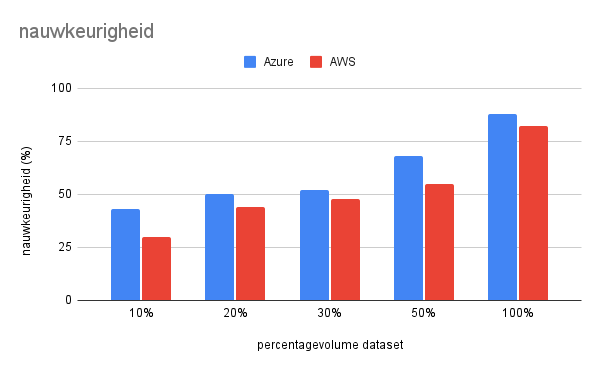
\includegraphics[width=0.75\textwidth]{nauwkeurigheid}
\end{figure}

\begin{figure}[h]
    \caption{Bar chart die de gewogen nauwkeurigheden van AWS en Azure vergelijkt per percentage van de dataset dat werd gebruikt als trainingsdata.}
    \centering
    \label{gewogen_nauwkeurigheid_chart}
    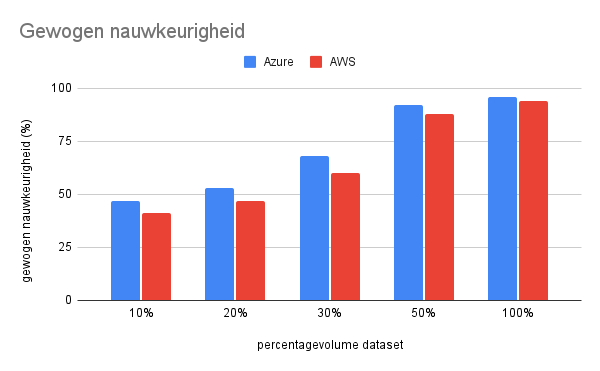
\includegraphics[width=0.75\textwidth]{Gewogen nauwkeurigheid}
\end{figure}

De gewogen nauwkeurigheid bereikt reeds 92\% wanneer 50\% van de originele dataset wordt gebruikt als trainingsdataset. 

\section{Beslissen}
\subsection{Proof of Concept}
De eerste vraag die moet worden gesteld is of de modellen die zijn gegenereerd überhaupt zouden kunnen helpen bij het on-boarding proces van een nieuw PIM-systeem. Het is duidelijk dat voor beide providers de modellen die gegeneerd werden op basis van de datasets die respectievelijk 10\%, 20\% en 30\% van de originele dataset bevatten, zeker niet geschikt zijn voor het autonoom toevoegen van tags aan de entiteiten van het systeem. Zowel het model van Azure als het model van AWS die met 50\% (350 records) van de originele dataset werden gegenereerd zijn zeker geschikt voor het geven van gerichte suggesties, en eventueel ook al voor het zelfstandig taggen van entiteiten. Beide modellen die werden gegenereerd met de originele dataset zijn zeker geschikt voor het geven van suggesties en ook voor het zelfstandig taggen. Dit wil zeggen dat het integreren van Machine Learning in het taxonomie systeem van PIMLayer zou kunnen helpen bij zowel het onboarding proces als bij het onderhouden en updaten van een bestaand PIM-systeem. Dat laatste is ook interessant voor andere PIM-systemen, zoals het systeem waar de Constructalia-dataset werd uit gehaald. 
\subsection{AWS of Azure}
Voorlopig gebruikt PIMLayer geen specifieke AWS of Azure producten. De snelheid van de services van de providers spelen in deze geen rol, aangezien het vaak gaat over buffer operaties met een lage prioriteit (zeker in het onboarding proces). Dat wil zeggen dat we ons kunnen beperken tot de resultaten en de prijs om een beslissing te nemen tussen beide providers. 
Aangezien Azure betere resultaten kan neerleggen voor elke train-dataset en er een goedkopere configuratie kan worden gemaakt op Azure is de keuze voor Azure de logische. 


\section{Toegevingen}
\subsection{1 model per tag}
De modellen die in dit onderzoek worden gegenereerd kunnen slechts 1 tag voorspellen, terwijl PIMLayers tag-systeem meerdere soorten tags ondersteunt. Dit wil zeggen dat er voor elke tag een ander model zou moeten worden gegenereerd, en dat ook nog eens voor elke klant. Het zou dan ook interessant kunnen zijn om de eindgebruiker te laten instellen voor welk type tags er een model moet worden voorzien en voor welke niet.

\subsection{Meerdere tags binnen dezelfde groep}
Het taxonomie systeem van PIMLayer ondersteunt ook meerdere tags per bestand, de modellen die voor dit onderzoek zijn gegenereerd konden hier moeilijk mee om, zo bleek uit de zoektocht naar welke tag de modellen zouden moeten gaan voorspellen. Misschien is het mogelijk om de gegeneerde modellen zodanig aan te passen opdat ze hier wel mee kunnen omgaan.  

\subsection{Negatieve feedbackloop}
Hoe kan ervoor worden gezorgd dat het model blijft bijleren? Zou het mogelijk zijn om een negatieve feedbackloop toe te voegen aan de modellen zodat het voorspellend vermogen van een model toeneemt? 

\section{Verder onderzoek}
Nu er een keuze kan gemaakt worden qua provider is de volgende uitdaging om deze te integreren in PIMLayer zelf. Er moet ook nog nagedacht worden over hoe en op welke manier dit zou moeten gebeuren...

% TODO: Trek een duidelijke conclusie, in de vorm van een antwoord op de
% onderzoeksvra(a)g(en). Wat was jouw bijdrage aan het onderzoeksdomein en
% hoe biedt dit meerwaarde aan het vakgebied/doelgroep? 
% Reflecteer kritisch over het resultaat. In Engelse teksten wordt deze sectie
% ``Discussion'' genoemd. Had je deze uitkomst verwacht? Zijn er zaken die nog
% niet duidelijk zijn?
% Heeft het onderzoek geleid tot nieuwe vragen die uitnodigen tot verder 
%onderzoek?





%---------- Bijlagen -----------------------------------------------------------

\appendix

\chapter{Onderzoeksvoorstel}

Het onderwerp van deze bachelorproef is gebaseerd op een onderzoeksvoorstel dat vooraf werd beoordeeld door de promotor. Dat voorstel is opgenomen in deze bijlage.

%% TODO: 
%\section*{Samenvatting}

% Kopieer en plak hier de samenvatting (abstract) van je onderzoeksvoorstel.

% Verwijzing naar het bestand met de inhoud van het onderzoeksvoorstel
%---------- Inleiding ---------------------------------------------------------

\section{Introductie}%
\label{sec:introductie}

PIM (Product Information Management) systemen zijn alomtegenwoordig in de e-commerce wereld. Ze focussen op het onderhouden, verrijken en beheren van alle info die te maken heeft met de producten van een bedrijf. Het doen van dit proces is het creëren van een single source of truth, die dan kan gebruikt worden voor sales en marketing doeleinden. \autocite{Matilla2018}

PIMLayer een Gents bedrijf dat PIM-systemen aanbiedt. Hun implementaties werken met een taxonomie systeem dat toelaat om elk product en item op verschillende en meerdere niveaus van tags te voorzien. \autocite{AwareNV2022} Dit systeem zorgt ervoor dat de gebruiker heel specifieke en performante query's kan opstellen binnen het systeem. Een gebrek van deze feature is dat alle tags door de gebruiker zelf moeten worden toegevoegd aan alle producten en items in het systeem.


De oplossing voor dit probleem zou een slimme onboarding tool zijn die, gebruik makend van Machine Learning, slimme suggesties kan doen voor de tags die bij een bepaald item of product horen op basis van de data die al aanwezig is in het PIM systeem, en op termijn misschien zelfs zelfstandig tags kan toevoegen. De implementatie van de tool zou gebruik maken van een MLaaS (Machine Learning as a Service)  Het doel van deze bachelorproef is om 3 verschillende aanbieders van MLaaS: Amazon Machine Learning services, Microsoft Azure Machine Learning Studio en Google Cloud Platform, te vergelijken op basis van hoe snel ze een bepaald succespercentage kunnen behalen. 

Op basis van de resultaten van deze bachelorproef kan de best passende MLaaS worden geïntegreerd  in PIMLayer.



%---------- Stand van zaken ---------------------------------------------------

\section{State-of-the-art}%
\label{sec:state-of-the-art}

\subsection{Machine Learning}
\textcite{Hu2013} beschrijft het doel van machine learning als het ontwerpen en ontwikkelen van algoritmes die systemen toelaten om op basis van data, ervaring en training zichzelf aan te passen. 
\subsubsection{Algoritmes}
Machine learning algoritmes kunnen worden verdeeld op basis van hoe hun proces er uitziet :
\begin{itemize}
	\item \textbf{Supervised Learning}: het algoritme krijgt een gelabelde dataset om te trainen, op basis daarvan wordt een model opgebouwd dat niet gelabelde datasets kan classificeren. Achteraf moet een 'supervisor' hoeveel procent van de toegekende labels correct waren. 
	\item \textbf{Unsupervised learning}: het algoritme vertrekt vanuit een niet gelabelde dataset en gaat zelf op zoek naar patronen in de dataset. Op basis van de patronen maakt het algoritme zelf een classificatie.
	\item \textbf{Semi-supervised learning}: een hybride van supervised en unsupervised learning.
	\item \textbf{Reinforcement learing}: het algoritme leert hoe het zich moet gedragen op basis van een gegeven feit. Elke actie heeft een invloed op het model, dat op zijn beurt kan terugkoppelen naar het model om zo het gedrag te beïnvloeden.
	\item \textbf{Transduction}: gelijkaardig aan supervised learing, maar genereert niet per se een functie, het probeert de nieuwe outputs te voorspellen op basis van training inputs, training outputs en nieuwe inputs.
	\item \textbf{Learning to learn}: het algoritme leert zichzelf gedrag aan gebaseerd op vorige ervaring.
\end{itemize}
\autocite{Zhang2010}


\subsubsection{Machine Learning as a Service (MLaaS)}
MLaaS is de verzameltern voor de verzameling van cloud-based platforms die machine learing gebruiken om oplossingen aan te bieden. \autocite{Onose2022}. Deze oplossing kunnen meerdere vormen aannemen: 
\begin{itemize}
	\item voorspellende analyse voor verschillende use cases
	\iten trainen en afstellen van een model
	\item implemenatie van een model
\end{itemize}

MLaaS heeft ook een aantal gebreken, zo heb je zelf niet altijd controle over de gebruikte algoritmes en parameters en het is niet geschikt voor gevoelige data.

\subsubsection{eerder onderzoek}
\textcite{Madhuri2016} stelt dat de verschillen tussen Amazon Web Services (AWS) en Microsoft Azure klein zijn en dat de keuze voor de ene of de andere optie neerkomt op use-case en eigen voorkeur. \textcite{Pinto2018} gebruikte de volgende criteria om MLaaSes te vergelijken :
\begin{itemize}
	\item schaalbaarheid
	\item snelheid
	\item in welke mate dient de oplossing zijn oorspronkelijke doel
	\item bruikbaarheid
\end{itemize}
\textcite{Pallavi2020} vergeleek de AWS, Google en Azure oplossingen op algemeen vlak, en dus niet voor een specifieke usecase, maar concludeerde net als \textcite{Madhuri2016} dat de keuze afhankelijk is van de use-case en eigen voorkeur.

Uit \textcite{Pallavi2020} en \textcite{Madhuri2016} kunnen we volgende tabel besluiten: 
\begin{itemize}
	\item schaalbaarheid en het ondersteunen van meerdere SQL-varianten zijn de grootste troeven van AWS
	\item het feit dat Azure gemakkelijk in te passen is in een reeds bestaande Microsoft omgeving is een grote troef van Azure
	\item Google maakt gebruik van de meest performante systemen om zijn berekeningen te doen en heeft veel ingebouwde libraries
	\item Azure ondersteunt alleen AzureSQL
\end{itemize}


\subsection{PIM}
Het belang van Product Information Management (PIM) stijgt door het alsmaar verhoogde niveau van de technische complexiteit  van producten, die complexiteit zorgt ervoor namelijk voor dat er een overvloed aan informatie ontstaat die bovendien moeilijk up-to-date kan worden gehouden. \autocite{Fr_mling_2006} Vaak combineert een PIM-systeem data uit verschillende andere systemen en databronnen (zoals ERP's, databanken, excels, etc.) en bundelt het die tot een single-source of truth die bovendien altijd up-to-date is. De data van het PIM-systeem kan dan worden geconsumeerd door brand portals, product sheets, een webshop, ...



%---------- Methodologie ------------------------------------------------------
\section{Methodologie}%
\label{sec:methodologie}

Er wordt vertrokken vanuit een dataset van ongeveer 40 000 records, deze omvatten zowel entiteiten als assets (text-based) uit een reeds bestaand PIM-systeem. Hiervan beschouwen we de eerste 90\% als data die gebruikt mag worden om te trainen en de laatste 10\% als controle data. De controle data zal gebruikt worden om de nauwkeurigheid van de oplossing te testen. Om ervoor te zorgen dat we niet eindigen met de 4000 recentste records, waar nieuwe trends of fenomenen zich kunnen voordoen, halen we elk 10de record uit de dataset en voegen we deze toe aan de controle data.
Om de 3 opties te vergelijken, zullen de volgende stappen voor alle opties worden doorlopen:

\begin{enumerate}
	\item opzetten van een account
	\item configuratie van infrastructuur
	\item opladen van 10\% van de dataset
	\item laten ontwikkelen van oplossing
	\item testen van huidige oplossing tegen de controle data
	\item stappen 3) en 4) hernemen voor 20\%, 30\%, 40\%, 50\%, 60\%, 70\%, 80\% en 90\%
\end{enumerate}

Door verschillende percentages van de dataset te gebruiken krijgen we een beter zicht op de leercurve van een oplossing.

Hierna kunnen we de 3 opties vergelijken op: 
\begin{itemize}
	\item aantal records die de tool nodig heeft om een nauwkeurigheid van meer dan 50\%, 75\% en 90\% te bereiken
	\item tijd die de tool nodig heeft om een oplossing op te stellen
	\item evolutie verhouding tussen aantal records die te tool nodig had om te trainen en nauwkeurigheidspercentage
	\item tijd die tool nodig heeft om de controle data te verwerken (en eventueel of die verandert naarmate er meer data naar de tool wordt opgeladen).
	\item gebruiksvriendelijkheid van de tool en eventuele extra features, dit kan door het meten van de tijd die nodig is om een account aan te maken of om de omgeving te configuren.  
	\item prijs
\end{itemize}

Op basis van die vergelijking kan dan een keuze worden gemaakt voor de beste tool.

%---------- Verwachte resultaten ----------------------------------------------
\section{Verwacht resultaat, conclusie}%
\label{sec:verwachte_resultaten}

Er wordt verwacht dat de 3 tools niet significant zullen verschillen in performantie, de doorslaggevende factor(en) zullen dan waarschijnlijk prijs en gebruiksvriendelijkheid van de tool zijn. Het zou ook kunnen dat eventuele marketing doeleinden ook een rol spelen in de eindbeslissing. Amazon Machine Learning services bieden de meeste en meest geavanceerde extra-functionaliteiten aan en zijn ook zeer attractief op vlak van prijs. 

%%---------- Andere bijlagen --------------------------------------------------
% TODO: Voeg hier eventuele andere bijlagen toe. Bv. als je deze BP voor de
% tweede keer indient, een overzicht van de verbeteringen t.o.v. het origineel.
%\input{...}

%%---------- Backmatter, referentielijst ---------------------------------------

\backmatter{}

\setlength\bibitemsep{2pt} %% Add Some space between the bibliograpy entries
\printbibliography[heading=bibintoc]

\end{document}
